\documentclass[sigconf,10pt,nonacm]{acmart}

\settopmatter{printacmref=false} % Removes ACM reference format


\usepackage[utf8]{inputenc} % allow utf-8 input
\usepackage[T1]{fontenc}    % use 8-bit T1 fonts
\usepackage{hyperref}       % hyperlinks
\usepackage{hyperref}
\hypersetup{
    colorlinks=true,
    linkcolor=blue,
    filecolor=blue,      
    urlcolor=blue,
    citecolor=blue
}
\usepackage{url}            % simple URL typesetting
\usepackage{amsfonts}       % blackboard math symbols
\usepackage{nicefrac}       % compact symbols for 1/2, etc.
\usepackage{microtype}      % microtypography
\usepackage{xcolor}         % colors
\usepackage{enumitem}
\usepackage{authblk}

% Libraries for Giant Table
\usepackage{array}
\usepackage{amsmath}
\usepackage{booktabs}       % professional-quality tables
\usepackage{changepage}
\usepackage{multirow}
\usepackage{wrapfig}
\usepackage[small, compact]{titlesec}

\usepackage[font={small}]{caption}
\usepackage[export]{adjustbox}
\usepackage[skip=1ex]{caption}

% basics
\newcommand{\handlemath}[1]{\relax\ifmmode #1\else $#1$\fi}
\newcommand{\figref}[1]{{Figure~\ref{#1}}}
\newcommand{\secref}[1]{{\S\ref{#1}}}
\newcommand{\eg}{e.g., }

% Superscript command
\newcommand{\tss}[1]{{\textsuperscript{#1}}}

% comments, etc.
\newcommand{\todo}[1]{}
\newcommand{\cjr}[1]{}
\newcommand{\ds}[1]{}
\newcommand{\aditya}[1]{}
\newcommand{\jane}[1]{}
\newcommand{\rohit}[1]{}
\renewcommand{\todo}[1]{{\color{blue}\textbf{TODO:} #1}}
\renewcommand{\check}[1]{{\color{orange}\textbf{Check:} #1}}
\renewcommand{\cjr}[1]{{\color{red}\textbf{[cjr]:} #1}}
\renewcommand{\ds}[1]{{\color{teal}\textbf{[ds]:} #1}}
\renewcommand{\aditya}[1]{{\color{pink}\textbf{[aditya]:} #1}}
\renewcommand{\jane}[1]{{\color{olive}\textbf{[jane]:} #1}}
\renewcommand{\rohit}[1]{{\color{yellow}\textbf{[rohit]:} #1}}


%% A dense itemize environment
\newenvironment{denseitemize}{
\begin{itemize}[noitemsep, topsep=0pt, leftmargin=1.2em]
}{\end{itemize}}

 %% A dense enumerate environment
\newenvironment{densenumerate}{
\begin{enumerate}[noitemsep, topsep=0pt, leftmargin=1.2em]
}{\end{enumerate}}

% Reduce spacing after headings
\titlespacing*\section{0pt}{0pt plus 2pt minus 2pt}{0pt plus 2pt minus 2pt}
\titlespacing*\subsection{0pt}{0pt plus 2pt minus 2pt}{0pt plus 2pt minus 2pt}
\titlespacing*\subsubsection{0pt}{0pt plus 2pt minus 2pt}{0pt plus 2pt minus 2pt}

\makeatletter
\renewcommand\AB@affilsepx{, \protect\Affilfont}
\makeatother

\title{How I {\it learned} to not worry about {\it learned} policies in my OS}

% The \author macro works with any number of authors. There are two commands
% used to separate the names and addresses of multiple authors: \And and \AND.
%
% Using \And between authors leaves it to LaTeX to determine where to break the
% lines. Using \AND forces a line break at that point. So, if LaTeX puts 3 of 4
% authors names on the first line, and the last on the second line, try using
% \AND instead of \And before the third author name.

\begin{abstract}
Operating System policies are becoming increasingly workload-dependent, where assumptions about workloads, application behavior, and hardware shape policy design. When these assumptions fail to hold in deployment, policies can silently degrade performance.
Existing engineering practice relies on offline benchmarking, which is ill-suited to addressing deployment-time performance regressions and provides little insight for future policy iterations. 
This paper argues that OSes need \emph{performance introspection}: the ability to monitor \emph{during execution} whether a policy is satisfying its performance requirements, and---crucially---to intervene when it is not.
To this end we propose the abstraction of \emph{OS guardrails}, which pair (i) a runtime-checkable performance condition with (ii) a corrective action.
We present principles for designing useful guardrails, a Guardrail Description Language (GDL) and semantics for specifying guardails over kernel-visible signals, an implementation substrate based on in-kernel monitors and eBPF, and a verification interface for verifying that local guardrail conditions (and their corrective actions) ensure system-wide performance objectives.
We demonstrate the effectiveness of this approach through five case studies, showing that guardrails expose broken deployment-time assumptions, surface policy-specific failure modes, and enable targeted corrections or safer fallbacks.
\end{abstract}

\begin{document}

\maketitle
\section{Introduction}\label{sec:introduction}
\cite{climax-icml-23}
\section{Motivation}\label{sec:background}\label{sec:motivating}

%\aditya{is this a motivation for why we need guardrails or for our design of guardrails? accordingly, make the section title precise}
%\sujay{I have attempted to make the first part about why we need guardrails. And the second part about design of guardrails.}

Traditionally, OS policies are designed to perform well across a broad range of workloads and hardware configurations. However, growing workload diversity and hardware heterogeneity have driven increasing interest in designing policies tailored to specific deployment contexts to achieve better performance.
Recent research has focused on enabling customization of OS policies using eBPF~\cite{sched-ext,cache-ext-sosp25,pageflex2025}, tuning OS parameters per workload~\cite{tuning-pacmi25,agentic-tuning-ml4sys25}, and developing learned policies~\cite{heimdall-eurosys25,orca-sigcomm20,kml-tos23,kleio-hpdc19,linnos-osdi20}. More recently, researchers are leveraging AI agents to generate specialized heuristics~\cite{policysmith-hotnets25,glia-arxiv25,barbarians25,vulcan-arxiv25,agentic-os-ml4sys25}.
Whether traditional or specialized, all these policies share a common limitation: developers typically evaluate them on a limited set of benchmarks before deployment, with no mechanism to verify that the policy continues to meet its performance goals during runtime.

% Typically, OS policies are designed to achieve performance requirements such as increased throughput or reduced latency. Standard practice is to justify those requirements empirically using offline benchmarks. This statistical evidence is limited by the workloads and environments on which the policy was evaluated, and those assumptions have proven not to hold in in deployed systems. For instance, the LinnOS~\cite{linnos-osdi20} system predicts I/O latency from request and device features, trained on a specific class of devices; However, the latency accuracy degrades when deployed on faster devices~\cite{heimdall-eurosys25}.

\subsection{Brittle Assumptions in Modern OS Policies}

\begin{figure}[t]
    \centering
    \setlength{\belowcaptionskip}{-10pt}
    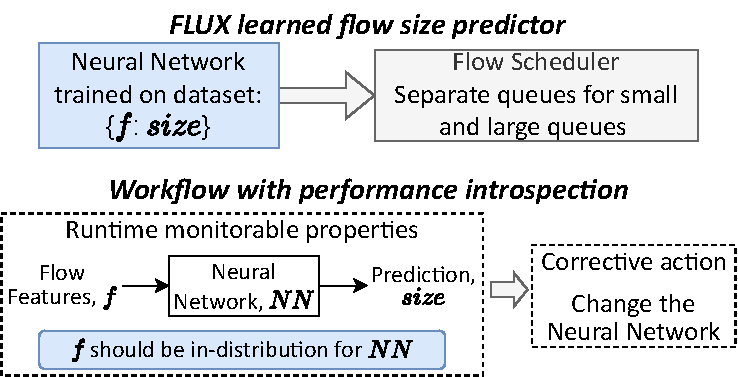
\includegraphics[width=0.7\columnwidth]{figures/Examples/FLUX-example.pdf}
    \caption{A common challenge: learned predictors care about good accuracy, but fixing performance degradations requires constant offline retraining. Instead, we propose run-time checks using observable proxies such as input-distribution checks.}
    \label{fig:flux-example}
\end{figure}

\begin{figure}[t]
    \centering
    
    \setlength{\belowcaptionskip}{-10pt}
    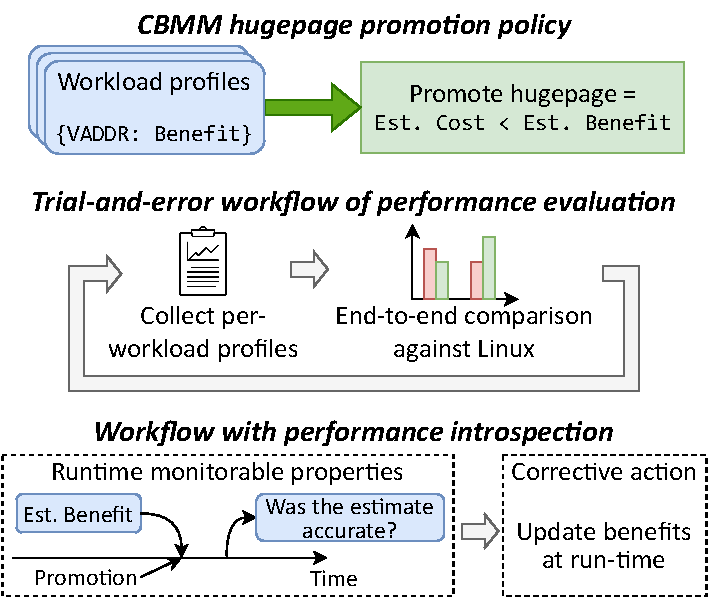
\includegraphics[width=0.7\columnwidth]{figures/Examples/CBMM-example.pdf}
    \caption{CBMM illustrates an additional challenge: the policy cares about correctness of promotion decisions, but any run-time check must rely on currently observable signals.}
    \label{fig:cbmm-example}
\end{figure}

We provide two examples to demonstrate how policies designed under certain assumptions or conditions can fail when those assumptions break at deployment time.

\noindent
{\it \textbf{Learned Flow Scheduling using FLUX.}}
% Learned predictors often perform well on in-distribution workloads but can degrade substantially under out-of-distribution ones.
Policies tuned or trained offline can silently degrade when deployment conditions or assumptions diverge from what they were built for.
Consider the FLUX learned flow scheduler~\cite{flux-nsdi19} (see \Cref{fig:flux-example}), which aims to reduce flow completion times. FLUX learns a model that predicts the completion time of a flow $f$ from a vector of run-time features $\vec v$, such as size and inter-arrival behavior, and uses these predictions to prioritize flows with smaller predicted completion times.
We observe that FLUX provides 75\% accuracy on large flows that match its training distribution, but degrades substantially (resulting in mere 21\% accuracy) on smaller flows that fall outside it. 
Unfortunately, the scheduler has no means to detect that the model has become unreliable and continues to use its predictions. 
% \sujay{@Divyanshu add numbers}

\noindent
{\it \textbf{Hugepage promotion in CBMM.}}
Even policies that are not learned can embed offline assumptions that silently break at deployment time. A concrete example arises in hugepage promotion.
Hugepages reduce TLB misses and address-translation overhead, but promoting them also incurs allocation and compaction costs and can increase memory bloat.
CBMM~\cite{cbmm-atc22} addresses this tradeoff by promoting a region only when an estimated promotion benefit exceeds an estimated promotion cost (see \Cref{fig:cbmm-example}), where the benefit estimates are profiled offline and the costs are derived from current system state. But, as workloads drift, those profiled benefit estimates may no longer reflect deployment-time behavior.

Such performance degradations are not uncommon -- they arise throughout the OS, from heuristic-based eviction policies for the page cache~\cite{cache-ext-sosp25} to learned I/O admission control for storage arrays~\cite{linnos-osdi20}.
In all of the above examples, the common practice for developers or infrastructure operators is to fall back on offline evaluation across a range of workloads (as shown in \Cref{fig:cbmm-example,fig:flux-example}), followed by manual inspection of end-to-end performance metrics.
This process is tedious, incomplete, and ultimately unsatisfactory: no finite offline evaluation can anticipate the diversity of executions encountered in deployment.

These examples motivate the need for a common framework for monitoring policy behavior at runtime and responding when they perform poorly. However, doing so requires overcoming fundamental challenges. % discussed below.

\subsection{Challenges with Runtime Monitoring}
The central challenge is determining what performance properties to monitor during runtime. Operators typically reason about high-level objectives such as tail latency, completion times, or eventual properties such as fairness. However, these metrics are not always observable within the OS.
A runtime monitoring system must therefore work with signals that the OS can observe, even when the operator's true objective lies outside the kernel's visibility. This raises another question: how can a local, kernel-observable property provide meaningful assurance about a high-level objective?

The CBMM example from \Cref{fig:cbmm-example} illustrates this tension concretely. The main objective of CBMM policy is that the promotion decisions should not degrade significantly relative to the decisions one would make using the true runtime benefits. Unfortunately, that objective is not directly observable at promotion time, because the true benefit of a promotion depends on future accesses.
What the OS can monitor, however, is whether stored benefit estimates follow the same order as recent accesses for different page regions.
This property is useful because, under the assumption that true runtime benefit is monotone with observed accesses, access ordering serves as a proxy for true-benefit ordering. If the estimated-benefits then match the access ordering, then the policy is more likely to preserve the intended comparison between benefit and cost at promotion time. Therefore, if the two orderings diverge, the stored profile is likely stale. A corrective action can then update the estimated benefits to restore this alignment, thereby helping preserve the quality of the resulting promotion decisions.


% While the performance objective is directly monitorable. In FLUX, the high-level objective of low flow completion times remains directly observable after the fact: once flows complete, the system can measure realized flow completion times and determine whether FLUX is continuing to deliver low average $\mathsf{FCT}$. If not, the system can revert to a safer alternative such as the default Linux scheduler.
% In many cases, it might not be possible to monitor a user's high-level objective within the OS kernel because it does not have access to it. While the performance objective may not itself what the OS can check at the point where it must act, but there is a run-time signal that allows it to infer \emph{something useful} about that objective. For instance, if the requirement is that queueing delay remain below a target $D$, the OS need not measure delay directly: in a FIFO queue with occupancy $q$ and service rate at least $\mu_{\min}$, the waiting time satisfies $W_q \leq q / \mu_{\min}$. Thus, enforcing $q \leq \mu_{\min} D$ is sufficient to ensure $W_q \leq D$. 

% \paragraph{Directly Observable Performance Objectives.}
% In some cases, the performance objective is directly monitorable. For example, if the requirement is that a subsystem maintain queue occupancy below a bound, say $\forall q.\;\mathsf{occupancy}(q) < N$, then the relevant quantity is available on the execution path, and the OS can monitor it directly and intervene when the bound is exceeded. 

% Returning to the FLUX example, its high-level objective, (based on $\mathsf{FCT}$s) however, remains directly observable after the fact: once flows complete, the system can measure realized flow completion times and determine whether FLUX is continuing to deliver low average $\mathsf{FCT}$. If not, the system can revert to a safer alternative such as the default Linux scheduler.


% \paragraph{Indirectly Observable Performance Objectives}
% However, in many important cases, 
% The same pattern appears in other familiar settings. In real-time scheduling, nonnegative slack implies deadline feasibility; in memory allocation, maintaining free-memory watermarks implies avoidance of reclaim-induced stalls. In all of these cases, the system monitors a signal that is not the objective itself, but that nevertheless provides a principled basis for intervention.


\subsection{Lessons for a New Framework}\label{subsec:lessons}

The examples above point to a common lesson: whether or not the ultimate performance objective is directly observable, one can often identify useful signals that indicate whether a policy is still operating in the regime for which it was designed. Unfortunately, today, such signals are rarely utilized. In many cases, OS policy designers do not attempt to detect regime shift at all; in other cases, they must handcraft monitoring and recovery logic that is tightly coupled to a particular policy and therefore difficult to reuse~\cite{linnos-osdi20,llama-asplos20,ingens-osdi16,sol-asplos22}.

The central thesis of this paper is that this should not be left to ad hoc mechanisms. Detecting when a policy has drifted out of its intended regime, and reacting appropriately when that happens, should be a first-class OS capability. The OS should provide a unified framework for specifying which signals matter, monitoring them at low overhead, and triggering corrective actions when needed. The framework proposed in this paper provides this capability through intuitive specifications and efficient in-kernel enforcement.

Another lesson from these examples is that identifying useful run-time signals is only part of the problem: those signals must ultimately connect back to some {\em higher-level performance objective}, such as promotion decisions being accurate for CBMM.
More broadly, such performance objectives may also require multiple runtime monitors, each capturing a different aspect of whether the policies are behaving as intended.
In such cases, simply reasoning about how a single runtime signal leads to the performance objective is not enough. The framework should additionally support compositional reasoning about how {\em collections} of local checks and repairs are \emph{jointly sufficient} to achieve the higher-level objective. 


% More broadly, the proposed framework is not limited to settings in which a single signal directly exposes a single failure mode. Many important objectives require multiple signals, each capturing a different aspect of whether the policy is behaving as intended. In such cases, no single guardrail is sufficient in isolation. Instead, different guardrails may need to monitor different signals and trigger different corrective actions, each addressing a distinct way in which the policy can drift out of its intended regime. To tackle this more challenging setting, our framework supports compositional reasoning about \emph{collections} of guardrails, making it possible to show that these local checks and repairs are \emph{jointly sufficient} to achieve a {\em higher-level performance objective}. 

% Taken together, these examples suggest a simple taxonomy: Some performance objectives are directly observable during execution; some are not observable within a run at all; and many of the most important ones are only indirectly observable through run-time signals that support a principled inference about the true objective. What is missing today is a systematic way to express which signals should be monitored, what corrective action should follow when they indicate a problem, and why those local checks are sufficient for the end-to-end property the designer actually cares about.l

% \subsection{The Observability Gap}

% In simple cases, the OS can directly check whether a subsystem is meeting its performance requirements. If the requirement is that a subsystem keep queue occupancy, run-queue length, or compaction overhead below a bound, the relevant quantities are already present on the execution path or in kernel-maintained counters, then the OS can monitor those quantities online, and can intervene when those bounds are exceeded. In such cases, the run-time check can coincide directly with the performance objective itself.

% On the opposite extreme, the OS wants to ensure that the policy is performing as intended, but cannot check the relevant performance condition directly. For instance, in SRTF scheduling, the OS wants to ensure that the scheduler is correctly prioritizing short jobs, because knowing how long a job will take requires knowledge of the future. The OS cannot preemptively check whether the scheduler is prioritizing short jobs. In this case, the only solution is post-hoc monitoring: the OS can check after the fact whether the scheduler's decisions were good, but it cannot know at decision time whether they will be. In such cases, the run-time is necessarily decoupled from the performance objective itself.

% However, many relevant cases fall somewhere in between, where there are runtime-observable signals that are directly related to the performance objective, but that do not directly measure it. For example, in CB 

% but it cannot know at dispatch time which jobs are actually short. In CBMM, the OS wants to ensure that hugepage promotions are paying off, but it cannot know at promotion time how future accesses will unfold. In learned scheduling, the OS wants to ensure that the model is making good predictions, but it cannot know at decision time how the flow will behave or how the queueing interactions will evolve.

% The OS must rely on surrogates that stand in for the true objective.
% The observability gap is the mismatch between the performance property the designer ultimately cares about and the evidence the OS can access at the time intervention is needed. Some performance properties can be checked directly during execution using kernel-visible quantities such as run-queue lengths, queue occupancies, allocator latency, or CPU time spent in a subsystem. Others cannot. Whether a hugepage promotion will pay off depends on future accesses; whether a learned scheduler made a good decision may depend on an outcome that arrives only later; whether a policy improved application throughput or tail latency may require external or counterfactual information.

% This distinction is fundamental because the OS can intervene only on the basis of what it can observe online. When the desired objective is directly monitorable, the run-time check can coincide with the objective itself or with a close operationalization of it. When it is not, the policy must rely on run-time surrogates that stand in for the hidden objective. Performance then depends not only on the policy logic, but also on whether those surrogates continue to track what the system actually cares about.

% This section develops that point. We first contrast cases in which the relevant performance condition is directly monitorable with cases in which it is not. We then show that the same observability gap appears across several OS subsystems. Finally, we use this gap to motivate performance introspection: a framework in which the run-time check, the corrective action, and the connection to the higher-level objective are all made explicit.

% \subsection{Directly Monitorable Performance Objectives}
% At one end are objectives that the OS can evaluate directly. For example, if memory compaction should not impose excessive overhead, the kernel can measure time spent in {\tt compact\_zone()} over recent windows and can disable or throttle hugepage promotion when that bound is exceeded. In such cases, the monitored condition is already close to the true objective. The check is local, online, and does not require prediction or oracle knowledge.



% CBMM~\cite{cbmm-atc22} chooses hugepage promotions by comparing estimated benefit against cost. Part of this decision problem is visible online: the current cost of promotion depends on quantities such as free or zeroed pages and on current compaction behavior. The key benefit term is not. The relevant quantity is the future reduction in address-translation cost obtained while the region remains promoted, and that quantity depends on accesses that have not yet occurred. The condition the designer ultimately cares about, namely that the system promote a region only when its future benefit exceeds its cost, is therefore not directly checkable at the time the decision is made. A run-time mechanism must instead monitor a surrogate, such as whether recent access behavior continues to preserve the ranking implied by the stored benefit estimates. When that surrogate fails, the system has evidence not that the objective itself was directly observed, but that the proxy used to approximate it has drifted out of alignment with the current execution.



% \subsection{Indirectly Monitorable Performance Objectives}

% % \subsection{A Pervasive Observability Gap}

% % This structure is not specific to CBMM or to learned scheduling. {\tt cache\_ext}~\cite{cache-ext-sosp25} shows that the best page-cache eviction heuristic varies across workloads. The objective is end-to-end hit rate or throughput, but the kernel must make online decisions using local signals such as recency, frequency, and observed reuse. Similarly, LinnOS~\cite{linnos-osdi20} predicts I/O latency from request and device features, yet Heimdall~\cite{heimdall-eurosys25} later shows that predictor accuracy can degrade on faster devices. At dispatch time, the system can inspect current request state, but it cannot yet know the true service time that would validate the prediction. Across memory management, caching, storage, and learned scheduling, the same mismatch recurs: the quantity the designer cares about is often global, delayed, or workload-dependent, whereas the quantity the OS can test online is local and immediate.

% % This is the setting in which deployment-time assumptions matter. Profiles, predictors, and tuned heuristics are not problematic merely because they are specialized. They are problematic because each of them compresses a hard-to-observe objective into a run-time surrogate. A workload shift, feature-distribution shift, or hardware change breaks precisely that correspondence. What fails is often neither functional correctness nor the existence of a policy decision, but the relationship between the signals observed online and the objective the policy was meant to optimize.

% \subsection{Why This Calls for Performance Introspection}

% The consequence is that performance introspection cannot be reduced to generic end-to-end monitoring. Collecting throughput numbers or tail latencies after the fact can reveal that performance regressed, but it does not tell the system what it can check online, when it should intervene, or which local condition has ceased to track the intended objective. A practical mechanism must instead work with conditions that are evaluable inside the OS during execution, cheap enough to monitor continuously, and informative enough to support action.

% When the desired objective is directly monitorable, the run-time condition may coincide with the objective itself or with a close operationalization of it. When the objective depends on future, external, or counterfactual information, the run-time condition is necessarily a proxy. In that case, the central design question is not only what the policy is trying to optimize, but also which observable condition best indicates that the policy is still operating in the regime for which it was designed. The corresponding response must likewise be executable online: update a parameter, switch to another installed policy, or fall back to a safer default.

% Performance introspection makes this structure explicit. It requires the designer to state which run-time condition will be monitored, what corrective action is available when that condition fails, and, when the condition is only a surrogate, why maintaining or restoring it supports the higher-level objective. This is the role of guardrails. The next section presents a framework for expressing such guardrails, while later sections formalize how local run-time checks can be related to the global performance objectives that motivated them in the first place.

\section{Performance Introspection}\label{sec:overview}

\ds{Some parts of this section might need to be lifted into the Intro.}
Specialized OS policies can provide performance gains for specific contexts but pose the risk of silent performance degradations under contexts that deviate even slightly.
% The core challenge in enabling performance reliability for specialized OS policies today is the lack of performance signals in the OS.
Today, the only practical way for operators to build confidence in specialized OS policies \aditya{this is imprecise. what does build confidence mean? be clear about what operators are trying to do with specialized policies and what blind spots/issues they face when using them.} is through extensive offline evaluation across many workloads, followed by manual inspection of end-to-end performance metrics.
This process is expensive, incomplete, and ultimately unsatisfactory: no finite offline evaluation can anticipate the diversity of executions encountered in deployment.

We argue that ensuring performance reliability for specialized OS policies requires a different capability altogether: rather than relying solely on offline testing and analysis, the OS should be able to introspect whether its policies are behaving well {\it at run-time}, using signals available during execution, and intervene when they are not. We call this capability {\it \textbf{performance introspection}}.
In this paper, we propose a framework that brings such run-time performance introspection capabilities to the OS.
The key building blocks enabling this framework are {\it \textbf{OS Guardrails}}.

\aditya{i don't like the specialization story.
isn't any policy "specialized" by definition or design?
also, note that beyond 3.0 there is no mention of specialization, so why bring it up in the first place
just say that policies are brittle from a perf perspective because designers are forced to make assumptions about workloads, enviornments etc that easily break at deployment time or in production. thus we need a principled way of knowing when that's happening and taking appropriate actions.}

% In the rest of this section, we first describe the workflow for performance introspection in our framework, explaining the guardrail primitive (\Cref{subsec:framework}), and then provide a formal basis for how run-time guardrails can provide performance reliability (\Cref{subsec:formal-basis}).

% A very successful technique has been to use formal verifiers before being deployed~\cite{certikos-osdi16}, or offline testing approaches can provide coverage over contexts of interest for the given policy\ds{add testing based cites}.
% One straightforward way to enable runtime signals about OS performance would be to have applications communicate explicit information about their achieved performance. However, besides breaking the current application-OS interface, this approach has a major flaw: simply providing end-to-end application performance indicators leaves no way for the OS to figure out which policy to improve. 
% Thus, such signals neither use readily available statistics nor are they actionable.

\subsection{OS Guardrails}\label{subsec:guardrails-desc}

An OS Guardrail (or guardrail, for simplicity) is a construct that evaluates whether the execution of an OS policy meets the requirement of reliable performance.
A guardrail captures two things: (i) a performance property that should hold for a policy or subsystem, and (ii) a corrective action to take when that property is violated.
We provide an intuitive explanation here, and give a detailed formal definition in \Cref{sec:gdl}.

We use the term \emph{performance property} to denote a measurable \eric{safety?}predicate over policy execution in the OS.
Depending on the policy, this predicate may be expressed over the policy’s inputs, its outputs, or the resulting system state.
For instance, a hugepage allocator may target low allocation latencies (captured by execution time statistics); a network flow scheduler with a learned flow size predictor may require high prediction accuracy (captured by the immediate outputs of the predictor); and a memory tiering policy may require high DRAM bandwidth utilization (captured by system statistics that result from using the policy).
These examples demonstrate the same underlying idea: the OS should be able to determine, from run-time evidence, whether the policy is operating in a desirable regime.

Corrective actions similarly depend on the policy and the failure mode being guarded against.
For instance, if a hugepage allocator takes too long, then the action may be to revert to the basepage allocator; if a predictor for flow sizes is resulting in inaccurate outputs, then the action may be to retrain the existing model; and if the memory tiering policy has low DRAM bandwidth utilization, then the action may be to promote pages more aggressively. \aditya{all of these are reactive actions. shouldn't we have proactive ones that deny an action}


\subsection{Principles for Designing Useful Guardrails}\label{subsec:principles}

\ds{A high-level question that I haven't answered head on is: why should guardrails be separate and not a part of the policy itself. Suggestions?}
\eric{Can probably borrow some motivation from Aspect Oriented programming https://en.wikipedia.org/wiki/Aspect-oriented_programming}
\sujay{As discussed, guardrails are more of an enhancement than a safeguard. We should mention this here or elsewhere.}
Guardrails are as useful as the properties they monitor -- thus, designing good properties is key to building useful guardrails.
We propose two principles for designing useful guardrails:
\begin{densenumerate}
\item Properties must be based on performance signals observable at run time within the OS.
\item Properties should capture the absence of undesirable behavior rather than prescribe ideal behavior.
\end{densenumerate}

% There are two guidelines we propose to design good performance properties.
To illustrate these principles and provide justification for them, we use transparent hugepage promotion (THP) as a running example.
For a hugepage promotion policy, the goal is to decide which set of contiguous pages to promote into a hugepage and when. Hugepages help by reducing TLB miss rates and hence, save page walk cycles, but these savings must also be balanced against the overhead of allocating hugepages~\cite{cbmm-atc22}.
A common method of specifying performance targets today is via tail-latency SLOs, as follows: `the 99th percentile execution time for any given workload when running the new policy should be at most 100 milliseconds'.

However, a property on application tail-latency SLOs is difficult for the OS to evaluate: it requires application-visible metrics, that break the application-OS interface.
\sujay{Instead, the guardrail should monitor the hugepage allocator latency to ensure its below a threshold.}
More generally, a property is useful for run-time performance introspection only if the OS can evaluate it during execution.
This restriction leads us to the first principle above.
Note that this principle rules out performance specified using end-to-end objectives that require external measurement, or properties whose validation is inherently offline, such as eventual convergence guarantees or long-horizon notions of fairness.
Such properties are still important, but they cannot serve as the basis for run-time performance introspection.

The second problem with the SLO-based performance property is that the SLO thresholds must vary with the workloads.
Thus, specifying a threshold for `ideal' performance is difficult. \aditya{this example is unclear. it is not obvious what ideal and bad means in this case and why one is difficult vs the other.}
In contrast, it is often much easier to identify clearly undesirable behavior -- operators and OS policy developers can use their domain knowledge to express invariants such as `at least this behavior should not happen'. \aditya{this is an ill-formed phrase}
This illustrates our second principle above. \aditya{inline these explanations with the principles. easier to follow and tighter.} \eric{I think an example would also make this easier to follow}

Taking these guidelines into account, a more useful guardrail can then be designed by specifying poor behavior that should not occur in any THP policy.
For example, if a THP policy repeatedly allocates hugepages that are never accessed, then the cycles spent in allocating them are necessarily wasted (and hence, a signal of poor policy performance).

\begin{figure}
    \centering
    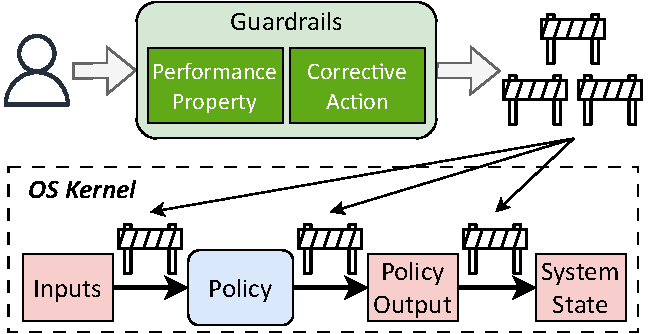
\includegraphics[width=0.9\columnwidth]{figures/Overview/overview.pdf}
    \caption{Overview of Guardrails}
    \label{fig:framework-overview}
\end{figure}

\subsection{Workflow and Key Components}\label{subsec:framework}

The above discussion shows that OS guardrails should be expressed as precise, executable specifications over OS-visible behavior.
This, in turn, imposes certain requirements needed to support performance introspection in the OS: guardrails must be specified declaratively, compiled into efficient monitors, and integrated directly into the execution path of OS policies.
We propose a framework that achieves these requirements. We explain this using the workflow depicted in~\Cref{fig:framework-overview}.

\aditya{the rest of this is good, but a bit verbose}
For each specialized policy (or subsystem) of interest, our framework requires operators to specify the guardrails, consisting of desired performance properties and corresponding corrective actions.
Today, there exists no mechanism for operators to specify the performance properties they require of the OS or the actions to take when the performance is poor.
The central challenge is therefore to provide an intuitive yet expressive interface for operators, while remaining implementable using run-time statistics.
Our framework addresses this challenge via the {\it \textbf{Guardrail Description Language (\lang)}}, a domain-specific language designed around typical OS abstractions such as kernel objects, kernel functions, and run-time statistics.
To ensure that properties can be evaluated at run time with low overhead, \lang uses primitives that restrict performance properties to predicates over kernel-visible features that are observable during execution (e.g., per-object counters, latency measurements, and scheduling or memory-state signals).

At run time, \lang guardrails are compiled into {\it \textbf{Guardrail Monitors}} that operate alongside the policy execution path, as depicted in Figure~\ref{fig:framework-overview}.
As inputs drive policy decisions and update system state, these monitors continuously evaluate the specified predicates over the resulting execution trace.
In order to make the varied statistics, necessary for evaluating properties, readily available, we maintain an in-kernel feature store, as proposed previously in LAKE~\cite{lake-asplos23}.
We implement these monitors using \texttt{eBPF}, enabling efficient in-kernel execution, low deployment overhead, and dynamic updates to guardrail logic.
When a predicate evaluates to false, the guardrail is said to be triggered, and this results in the execution of its prescribed corrective action, steering the policy back toward its intended operating regime.
\section{Discussion}\label{sec:discussion}

\ds{Performance introspection is the key idea -- runtime guardrails are one way to achieve it for a specific class of properties. Need to elaborate what properties these do not support, and what more would be needed.}
\section{Summary}\label{sec:summary}

We argued that OSes need \emph{performance introspection}: the ability to monitor whether a policy is still meeting its intended objective and to intervene when it is not. We introduced \emph{OS guardrails}, a framework that pairs run-time monitorable checks with corrective actions, supports explicit connection to higher-level objectives, and enables low-overhead enforcement. Across diverse case studies, guardrails exposed assumption failures, identified actionable causes of regressions, and enabled targeted corrections or safer fallbacks.

\bibliography{refs.bib}
\bibliographystyle{plainnat}

% \appendix

\iffinal
\section{Data Sources for OS Traces}\label{apdx:sources}
Below we list the various data sources that can be used to train \abbr{}:
\begin{denseitemize}
    \item \textit{Action logs from OS components:}  Kernel logs such as {\tt dmesg} in Linux/MacOS and event logs in Windows, 
    %when configured during boot, 
    capture kernel debugging data, hardware events (e.g., network link status), and system events like interrupts, process restarts. These logs capture the actions taken by the OS components and the system state used by OS tasks (System state and Actions columns in Table~\ref{tab:os_components}).
    % ~\cjr{Is it worth noting that dmesg is present in Linux and MacOS, but other OSes by necessity have similar tools (e.g. Windows has the Windows System Log.}
    % We can also get similar statistics on system calls and kernel data structures using eBPF~\cite{ebpf}.
    \item \textit{Resource metrics and hardware counters:} Hardware drivers record several quantities relating to the resource's state at a pre-configured frequency. These include CPU, memory, and disk bandwidth utilization, NIC queue length, and hardware counters. 
    %Frequently collected metrics from the hardware drivers about the state of the resource (e.g. CPU utilization, memory usage, disk bandwidth usage, NIC queue lengths, CPU hardware counters, etc.)
    \item \textit{Application workloads:} Workload traces from productions~\cite{alibaba-uservice-21, serverless-azure-20, borg-eurosys-15}, public infrastructures~\cite{taccstats} and synthetically generated ones offer detailed application-level information, such as application type, request arrival rates, statistics of resource usage during execution.
    % \item \textit{OS environment metadata:} This includes information about the hardware specifications \aditya{is it static info, or counters and other dynamic info like that?}\ds{mostly static -- but we need to collect traces on several environments is the point} of the system resources (e.g. CPU, Cache, RAM, NIC, file system, etc.) and the deployed environment (i.e. cloud server, robot, or edge server). This data directly reflects the Environment State column for the different OS tasks in Table~\ref{tab:os_components}.
\end{denseitemize}
\fi



\section{Decision Making Tasks in Operating Systems}\label{apdx:mdps}
\input{tables/os_components}

Table~\ref{tab:os_components} shows the various components in the OS and a \textit{representative subset} of the tasks for these components. It also shows the relevant system and environment states, action spaces, and the objectives of these tasks.
Each task description is also accompanied by an acronym that we use in the paper to refer to the particular task, e.g. \textbf{SCH} for the CPU scheduling task.


\iffinal
\section{Pretraining Methodology for \abbr{}}\label{apdx:pretrain}
We envision \abbr{} to be {\bf pre-trained} using self-supervised methods on a large corpus of OS traces. This pre-trained model would capture temporal relationships in the sequence of inputs it accepts and build an understanding of the system dynamics of the OS.
Existing literature (particularly in natural language) has proposed several pre-training tasks that can be used to develop this basic understanding. Notable among these are the Next Token Prediction~\cite{gpt-18}, Masked Language Modeling, Next Sentence Prediction~\cite{bert-18}; each with their own pros and cons.
While it seems intuitive to employ an auto-regressive model, pre-trained with next token prediction to build \abbr{}, the optimal pre-training task is an open and interesting question in itself.



\section{Open Challenges for \abbr{}}\label{apdx:challenges}
\subsection{Challenges in using \abbr{} as a Policy Agent}
End-to-end application performance depends on collective decisions made by OS components.
Using foundation models as policy agents brings two unique challenges:  \textit{composability} of actions from various policy agents and end-to-end \textit{explanability} of their decisions.
The former arises because decisions of one policy can affect the future states of other agents (as with the \textbf{CACHE} and \textbf{SCH} example discussed in \secref{sec:background}).
Independently fine-tuned components in the OS may result in suboptimal OS-wide decisions, that may affect both individual application and system-wide guarantees (e.g. fairness and starvation-freedom). 
% On the other hand, system-wide guarantees on decision quality and explanations for individual decisions necessitate a holistic understanding of OS behavior.
One possible approach here is to jointly fine-tune components (to ensure concerted decisions) as well as to develop techniques that provide component-wise guarantees (on performance, e.g., bounds on tail request completion times, or correctness, e.g., safety and liveness properties~\cite{whirl-sigcomm-21}), and \textit{formally guaranteed composability} of these actions to provide global invariants for the entire OS.

Regarding the latter, ideally, we desire human users to understand the OS at some level to audit or debug it. However, learned decisions from a black-box model may easily obscure the understanding of overall behavior.
We envision the use of approaches that describe what each learned policy did in a given execution (similar to LIME~\cite{lime-2016}), what could have happened had a learned policy made a different decision, and also produce human-comprehensible `summaries' in the form of rules~\cite{dillig-counterfactual-expl-icse-22,dillig-explaining-mispredictions-2021}, or programs~\cite{interpretable-icml-18-swarat} of what the module will do ahead of time.

\subsection{Challenges in using \abbr{} as a Generative Model}
As with any generative model, quantifying the quality of synthetic samples is a key challenge.
At the very least, these traces should
% closely match real trace distributions (e.g., request arrival and size patterns for a \textbf{CACHE} task trace must be similar to real-world traces) while maintaining
maintain certain relationships between variables (e.g., total network transmissions should be less than network bandwidth).
They must also capture desired properties that are difficult to obtain otherwise, such as `realism', i.e., a specific sequence of requests in a generated trace can actually arise in practice --- this is an avenue for future research.
Further, the generated traces should also be diverse to be useful. For example, for a cache replacement algorithm, we would want traces with diverse and realistic combinations of small and large object arrivals to effectively stress-test the algorithm~\cite{darwin-sigcomm-23}. 
% \dk{A sentence explaining the privacy challenge is gone. If it was intentional, I think we should remove the following sentences also.}\ds{I merged that in the following one - the following sentences capture the privacy challenge, no?}
Another challenge is with leakage and memorization of sensitive data. As shown in previous works~\cite{diffusion-sec-23,codex-sec-23}, carefully designed prompts can extract memorized training data with sensitive information. Thus, integrating techniques such as filtering the memorized data~\cite{llm-sec-21} and ideas from say, differential privacy~\cite{dp-tcc-06}, into \abbr{} are necessary.
\fi

%%%%%%%%%%%%%%%%%%%%%%%%%%%%%%%%%%%%%%%%%%%%%%%%%%%%%%%%%%%%


\end{document}